\chapter{Implementation} \label{implementation}
This chapter will elaborate on the test data used as well as the process that was followed to achieve the results in Chapter \ref{results}.
\section{Existing data}
The data used was acquired by \cite{Westhuyzen:2020} for an article assessing the charring rate of both SA-Pine and Eucalyptus.
	For the purpose of this project, only the data obtained from the SA-Pine test was considered and analysed. 
	\subsection{Summary of test}
	The test was conducted on a sample panel of $100$ mm by $0.9$ m $\times 0.9$ m cross-laminated SA-pine.
	This sample was then divided into nine cubes of $100$ mm $\times 100$ mm $\times 100$ mm.
	%The sample was a 100 mm by 0.9m x 0.9m panel of cross-laminated SA-pine, this sample was then divided into nine cubes of 100 mm x 100 mm x 100 mm.
	Each cube was fitted with seven Type K-thermocouples placed at consecutive $16.5$ mm drilled holes, as can be seen in Figure \ref{TC_layout}. 
	The test panel was tested in a furnace and was exposed to the standard ISO 834 Fire curve (Figure \ref{firecurve_fig} and Equation\ref{firecurve_eq}) on one side and room temperature on the other. 
	The panel was exposed to the fire curve for $50$ minutes, at which stage near complete de-lamination was observed and the test ended.
	\begin{figure}
	\centering
	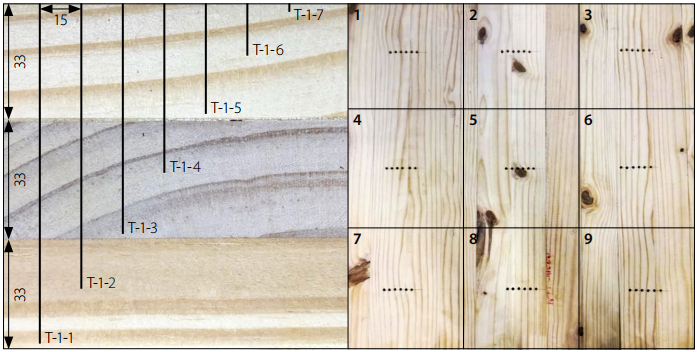
\includegraphics[width=\textwidth]{figures/TC_layout.png}
	\caption{Thermocouple layout in test conducted by \cite{Westhuyzen:2020} cross-section (left) and overall layout (right)}
	\label{TC_layout}
	\end{figure}
	\begin{equation}\label{firecurve_eq}
	T = 20 + 345\log_{10}(8t_{min}+1)
	\end{equation}
	\begin{figure}
	\centering 
	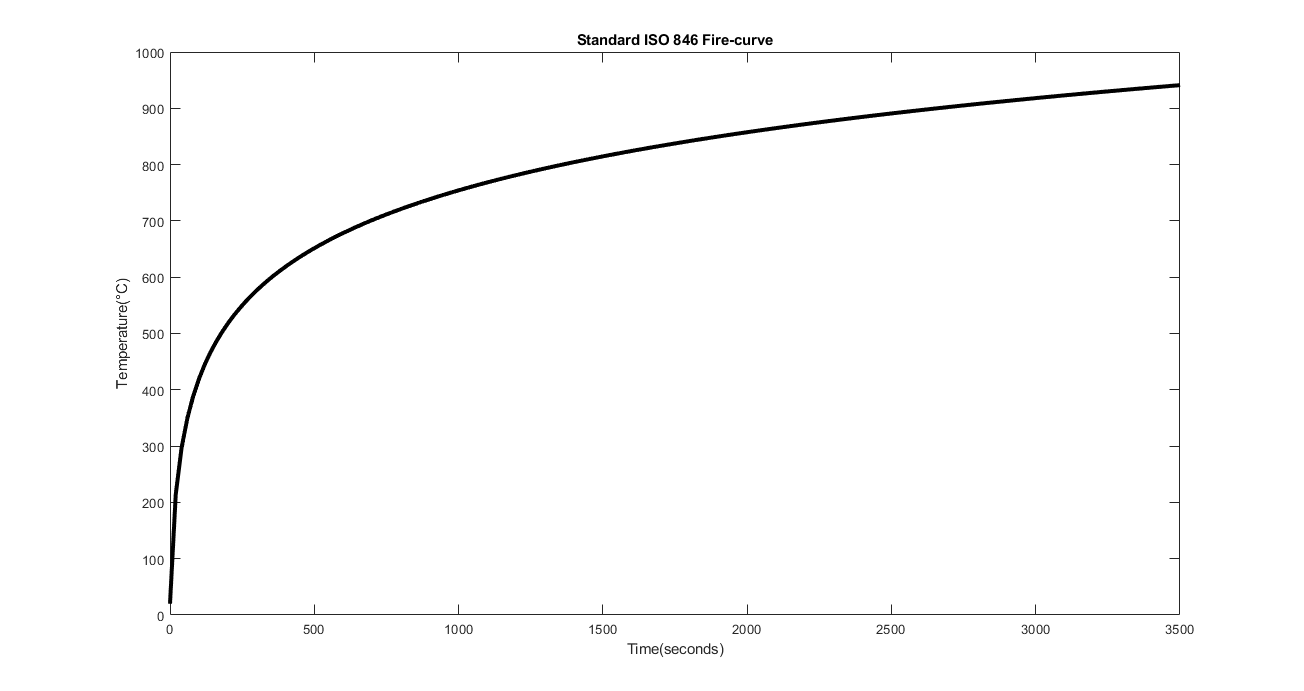
\includegraphics[width=\textwidth]{figures/firecurve.png}
	\caption{Standard ISO fire curve}
	\label{firecurve_fig}
	\end{figure}
	In Figure \ref{measured_fig} the measured temperatures at different depths in the sample can be seen. 
	These same depths will be used in the model and throughout the project to analyse the accuracy of the modelling that was done.
	\begin{figure}[H]
	\label{measured_fig}
	\centering
	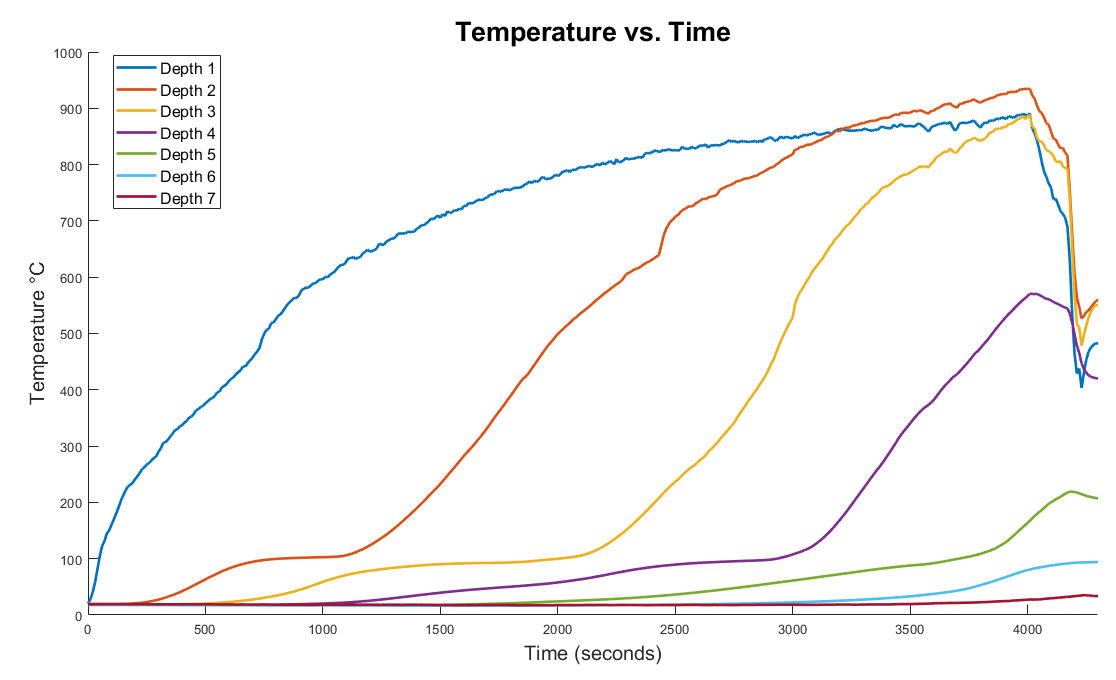
\includegraphics[width=\textwidth,]{figures/measured_plot.png}
	\caption{Average of measured temperatures at the different depths}
\end{figure}

	\subsection{Potential inaccuracies}
	As with most tests, everything is not always perfect. 
	The potential inaccuracies are discussed below. 	
	In the data, it was observed that two of the thermocouples malfunctioned during testing and could not be considered
	%; this resulted in temperature with a magnitude of $10^{13}$. 
	%Such a temperature is impossible, as the highest ever recorded temperature reached was $4\times 10^{12}$ and that only occurred in a atomic explosion. %(https://www.insidescience.org/news/hottest-temperature-universe-measured)% 
	This malfunction required that two of the depth measurements were no longer the average between nine samples but instead the average between eight.
	Another inaccuracy that could potentially influence the accuracy of the final result is the accuracy of the depth of the holes in which the thermocouples were placed. 
	%As this was done by hand in the laboratory.
	
	There is also debate about the significance of the contribution of the timber burning to the temperature inside the furnace. 
	For the purposes of this project, it will be assumed that the timber burning does not contribute to the temperature inside the furnace.
	
	
	
\section{Finite Element Modelling}\label{femexpl}
A one-dimensional finite element model that simulates what we expect to obtain from the fire tests based on the simplified $\kappa$-values provided in EN 1995:1-2-2004 \citep{Euro:2004} is modified into a function.
This function should provide the temperature of the modelled element based on a specified location and thermal conductivity.
The derivation and adaptation of the model are expanded on below.

\subsection{Existing Model}
	For this project, an existing finite element model of time-dependant conductive heat transfer implemented in Matlab by Prof. N de Koker was modified for usage in the Bayes' theorem~\ref{bayes_eq}. 
	This model is used to determine the likelihood function. 
	The current model uses the $\kappa$-values as well as the specific heat specified in EN 1995:1-2-2004. 
	 %shown in Equation \ref{cpusedeq}.
%\begin{equation} \label{cpusedeq}
%\centering
%  \texttt{cpine}=
%  \begin{blockarray}{*{14}{c} l}
%    \begin{block}{[*{14}{c}]>{$\footnotesize}l<{$}}
%      0 & 20 & 99&100& 120 & 121 & 200 & 250 & 300 & 350 & 400 & 600& 800 & 1200 \bigstrut[t]& $^{^\circ}\text{C}$ \\
%      479 & 479& 479 & 479 &  479 & 408 & 408 & 398 & 326&  220 &163 &  120 & 110 & 100 & $\text{kg/m}^3$ \\
%     1530 &1530 &1770 &13600& 13500& 2120& 2000& 1620 & 710 & 850 &1000& 1400 &1650& 1650 & J/kg/K \\
%    \end{block}
%  \end{blockarray}
%\end{equation}
	
	The model discretises the wooden element into 32 first order one-dimensional elements. 
	%For finite element analysis, there are always more elements used to generate the model than needed for evaluation. This is done to improve the accuracy of said model.
	This number of elements was sufficient to obtain converged results.
	The model is a one-dimensional finite element model that takes time differentiation into account.
	
\begin{figure}[H]
	\label{og_modeldata}
	\centering
	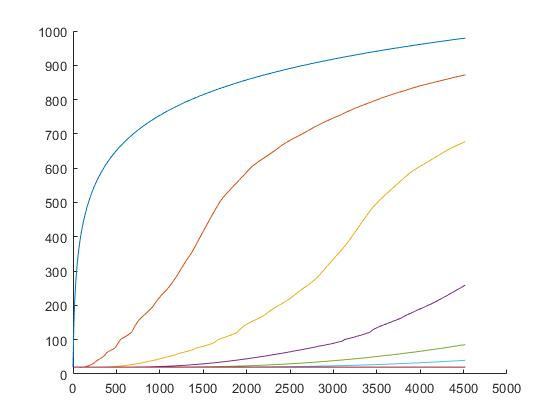
\includegraphics[width=\textwidth,]{figures/originalmugraph.jpg}
	\caption{Output of finite element model using $\kappa$-values as indicated in EN 1995:1-2-2004}
\end{figure}	

	\subsection{Derivation}%"CREATION?"
	%The assumption that the panel is constantly at room temperature on the outside is also inaccurate as there is heat radiating from the panel that increases the temperature surrounding the panel.
	
	Assumptions were made to simplify the model, they were as follows
	\begin{enumerate}
\item{The air on the side of fire follows the temperature of the fire curve.}
\item{The air on the cold side remains at 20\textdegree C.}
\item{The timber sample stays intact.}
\item{Thermal behaviour is isotropic throughout the model}

	\end{enumerate}
	\subsubsection{Stationary heat conduction}
	\begin{figure}[H]
	\label{femfig}
	\centering
	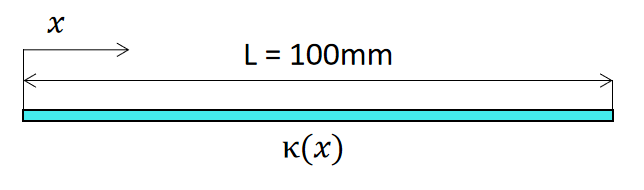
\includegraphics[width = 0.75\linewidth]{figures/fem_sketch.png}
	\caption{Visualisation of model in one-dimension}
	\end{figure}
	Based on \citet{Hughes:1987} and class notes from Informatics 314, the derivation started as a one-dimensional stationary heat conduction problem with the energy balance equation and the heat conduction equation.
	\begin{equation}
	\label{heateq1}
	q_{,x}-f = 0  \text{  ...(1)} \quad\quad\quad\quad q = -\kappa u_{,x} \text{  ...(2)} 
	\end{equation}
	Integrating Equation \ref{heateq1} (1) over the length of the element(shown in Figure \ref{femfig}) and introducing a weighting function $w(x)$ we obtain \ref{heateq2}. 
	Since the derivative of $w(0)$ is known and $q_{,x}$ is unknown. 
	The first term in \ref{heateq2} is integrated by parts. 
	After the integration by parts and substituting $q$ with \ref{heateq1} (2), Equation \ref{heateq3} is created.
	\begin{equation}
	\label{heateq2}
	\int_{x=0}^L wq_{,x}dx - \int_{x=0}^L wfdx = 0
	\end{equation}
	\begin{equation}
	\label{heateq3}
	\int_{x=0}^L wku_{,x}dx + \int_{x=0}^L wfdx - \left.wq\right|_0^L = 0
	\end{equation}
	In Equation \ref{heateq3} the $u$ and $w$ need to be defined.
	Assuming $u \approx u^h$ and $w \approx w^h$ and using the basis function ($N^A$), Equation \ref{basisfunc_eq} is obtained.
	\begin{equation}
	\label{basisfunc_eq}
	\begin{aligned}
	u_e^h = \sum_{B} N^B d^B  \quad &;\quad w_e^h = \sum_{A} N^A c^A\\
	u_{e,x}^h = \sum_{B} N_{,x}^B d^B \quad &;\quad w_{e,x}^h=\sum_A N_{,x}^A c^A\\
	\end{aligned}
	\end{equation}		
	Substituting the $u$ and $w$ functions back, we obtain the Galerkin weak form shown in Equation \ref{heateq4}.
	In Equation\ref{heateq4} the $A_N$ refers to the nodes that have Newmann boundaries ,explained in \ref{femsec}). 
	The variables $c^A$ and $d^B$ are independent of x and can therefore be taken out of the integral. 
	The sum over A and B are also taken out of the integral.
	After the summing is applied a matrix of all the possible combinations between A and B can be used to replace the sum. The resulting matrices are shown in Equation \ref{heateq5}. 
	When written in matrix form the summing is implied, if matrix form is not written then the expression referrers to the terms that will still be summed.

	\begin{equation}
	\label{heateq4}
	\begin{aligned}
	\sum_e \int_{\Omega_e} w_{e,x}^h k  u_{e,x}^h dx &+ \sum_e \int_{\Omega_e} w_e^h f dx - w(L)q_L + w(0)q_0 &= 0\\
	\int_{\Omega_e} \sum_A \sum_B N_{,x}^A c^A k N_{,x}^B d^B dx  &+ \int_{\Omega_e} \sum_{A} N^A c^A f dx - \sum_{A\in A_N} c^A q^A &= 0\\
	\end{aligned}
	\end{equation}
	\begin{equation}
	\label{heateq5}
	\vec{c}_e^T \vec{K}_e^{AB} \vec{d}_e + \vec{c}_e^T \vec{F}_e^f -\vec{c}_e^T \vec{F}_e^q
	\end{equation}
	where
	\begin{equation*}
	\begin{aligned}
	K_e^{AB} &= \int_{\Omega_e}N_{,x}^AN_{,x}^B k dx\\
	F_e^{Af} &= \int_{\Omega_e}N_{,x}^A f dx\\
	F_e^{Aq} &= \begin{cases} q(x_N) &\text{ for } x \in \Gamma_N\\0 &\text{ for other }\\
	\end{cases}
	\end{aligned}
	\end{equation*}
	
	\subsubsection{Boundaries} \label{airsec}
	\begin{figure}[H]\label{airelmfig}
	\centering
	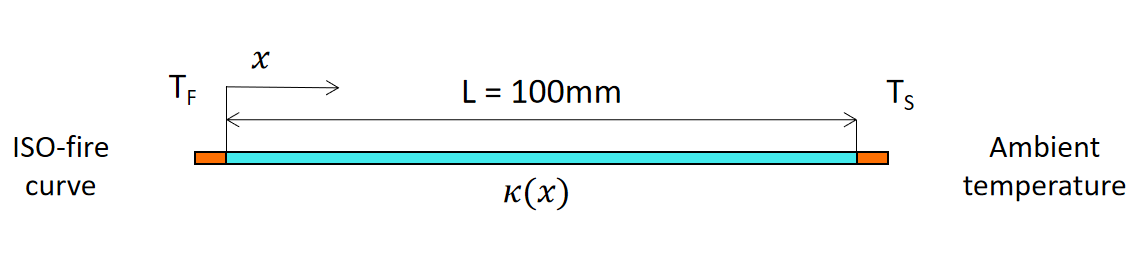
\includegraphics[width = 0.75\linewidth]{figures/fem_fire_sketch.png}
	\caption{Visualisation of one-dimensional model with air elements and external conditions added}
	\end{figure}
	
	One of the additional difficulties in modelling is that the known boundary temperatures are measured in the air of the furnace and assumed for the air outside the furnace.
	Initially, a long element of air was modelled.
	This element is then overlaid with the timber element to effectively add an air element it each end of the timber element as depicted in \ref{airelmfig}
	In the air elements, both heat convection and heat radiation need to be taken into account.
	The equations for heat convection and radiation can be seen in Equation \ref{heatconeq} and \ref{radeq}.
	
	\begin{equation} \label{heatconeq}       
	       \begin{aligned}
	       q_{\text{adv}}= \nu &\rho_A c_A \Delta T \quad = \quad h \Delta T\\	      
	       \nu =& \text{velocity m/s}\\
	       \rho_A =& \text{density of air}\\
	       c_{\rho} =& \text{heat capacity of air}\\
          \end{aligned}
	\end{equation}
	       
	\begin{equation} \label{radeq}
	       \begin{aligned}
	       q_{\text{rad}} = \varepsilon&\sigma \phi \left(T_f^4 - T_S^4\right)\\
	       \varepsilon =& \text{emissivity}\\
	       \sigma =& \text{Stefan-Boltzmann constant} \\&5.670 e^{-8} [W/(m^2K^4)]\\
	       \phi =& \text{view factor};1 \quad \text{here}\\
	       \end{aligned}
	\end{equation}
	Given that $T_S$ and $T_F$ are known a new equivalent heat flux value can be calculated as in Equation \ref{femboundeq1}.
	\begin{equation} \label{femboundeq1}
	q_{\text{con}}^{\text{equiv}} = \kappa^{\text{equiv}} \frac{\Delta T}{\Delta L} = q_{\text{rad}} + q_{\text{adv}}\\
	\end{equation}
	Due to the clear relationship between heat flux and thermal diffusivity the equivalent diffusivity($\kappa^{\text{equiv}}$) can be calculated as shown below in Equation \ref{femboundeq2}. 
	\begin{equation}\label{femboundeq2}
	\begin{aligned}
	\kappa^{\text{equiv}} &= \frac{\left[q_{\text{rad}} + q_{\text{adv}} \right]}{\Delta T}\\
	&\quad\\
	&= \frac{\epsilon \sigma \phi \Delta \left(T^4\right)}{\Delta T / \Delta L } + h \Delta L\\
	&\quad\\
	&= \frac{\epsilon \sigma \Delta \left(T^4\right)}{\Delta T   } + h\\
	\end{aligned}
	\end{equation}
	
	\subsubsection{One-dimensional diffusion}
The concept of heat diffusion is thoroughly explained in Section \ref{heatconsec} below the mathematical application is explained and steps that were taken to obtain the final model is shown.
	\begin{equation}\label{femdiffeq1}
	q_{,x} - f = \frac{\partial Q}{\partial t} = c_p \rho \frac{\partial u}{\partial t}\quad\text{  ...(1)} \quad\quad\quad q = -\kappa \frac{\partial u}{\partial x}\quad\text{  ...(2)}
\end{equation}
Substituting Equation \ref{femdiffeq1}(2) into \ref{femdiffeq1} and taking the derivative as indicated ($q_{,x}$) gives Equation \ref{femdiffeq2}. 
As previously discussed heat conduction ($\alpha$) is heat diffusion ($\kappa$)  divided by specific heat ($c_p$).


\begin{equation}\label{femdiffeq2}
\begin{aligned}
\therefore -\kappa \frac{\partial^2 u}{\partial x^2} - f &= c_p\rho \frac{\partial u}{\partial t} \rightarrow f=0:\\
\frac{\partial^2 u}{\partial x^2} &= - \frac{c_p\rho}{\kappa} \frac{\partial u}{\partial t} \quad \\
&\text{ or } \\
\frac{\partial u}{\partial t} &= -\alpha \frac{\partial^2 u}{\partial x^2}
\end{aligned}
\end{equation}


Let $c_p \rho = \lambda$ 

\begin{equation}\label{femdiffeq3}
\therefore -\kappa u_{,xx} - \lambda u_{,t} = f
\end{equation}


Then:

\begin{equation}\label{femdiffeq4}
\int_0^L w q_{,x} \text{d}x - \int_0^L w \lambda u_{,t} \text{d}x - \int_0^L w f \text{d}x = 0
\end{equation}


Similar to what was done in \ref{basisfunc_eq} a special approximation is made to obtain Equation \ref{femdiffeq5}.

\begin{equation}\label{femdiffeq5}
u \approx u^h \rightarrow u_e^h = \sum_{A}N^A d^A \quad;\quad w_e^h = \sum_{A}N^A L^A
\end{equation}


%\begin{equation}\label{femdiffeq6}
%\rightarrow \sum_e \int_{\Omega^e} w_{e,x}^h \kappa u_{e,x}^h \text{d}x_e + \sum_e \int_{\Omega^e} w_e^h \lambda u_{e,t}^h \text{d}x_e + \sum_e \int_{\Omega^e} w_e^h f \text{d}x_e - \sum_{e \in \epsilon_A} w q_N = 0
%\end{equation}
%
%\begin{equation*}
%*_1: \int_{\Omega^e} \sum_A \sum_B N_{,x}^A c^A \kappa N_{,x}^B d^B \text{d}x = \sum_A\sum_B \left[ \int N_{,x}^A N_{,x}^B \kappa \text{d}x  \right]d^B = \vec{c}_e^T \vec{\kappa}_e \vec{d}_e
%\end{equation*}
%
%
%\begin{equation*}
%*_2: \int_{\Omega_e} \sum_A \sum_B N^A c^A \lambda N^B \dot{d}^B \text{d}x = \sum\sum c^A \left[ \int N^A N^B \lambda \text{d}x \right] d^B = \vec{c}_e^T \vec{M}_e \vec{\dot{d}}_e
%\end{equation*}
%
%
%\begin{equation*}
%*_3: \int_{\Omega^e} \sum_A N^A c^A f \text{d}x = \sum c \int_B^A N f \text{d}x = \vec{c}_e^T \vec{F}_e^B
%\end{equation*}
%
%
%\begin{equation*}
%*_4: \sum_{A \in \mathcal{A}} \kappa^A q_N^A = \vec{c}_e^T \vec{F}_e^q
%\end{equation*}


From the above equations the below matrix formulation could be assembled:
%considere renamin to somehing with assembled or matrix in the name
\begin{equation}\label{femdiffeq7}
\vec{c}^T \vec{\kappa} \vec{d} + \vec{c}^T \vec{M} \vec{\dot{d}} = \vec{c}^T \vec{F}
\end{equation}

Where solving for $\vec{d}$ and $\vec{\dot{d}}$ is the main goal.
By setting $\vec{d}_0$ equal to the initial boundary conditions and setting $\vec{V}_0 = 0$ and integrating over time according to v-form time integration in Chapter 8 in \textit{The Finite Element Method} by \citeauthor{Hughes:1987} shown in detail in Appendix \ref{appder}.


Finally by combining the boundary conditions, stationary heat conduction and the one-dimensional heat diffusion models the below formulation in Equation \ref{solveeq2}.
\begin{equation}\label{solveeq2}
\vec{K}\cdot\vec{d} + \vec{M}\cdot\vec{\dot{d}} = \vec{F}' - \vec{F}^{Ke} - \vec{F}^{Me} = \vec{F}
\end{equation}

This can be solved as shown below in Equation \ref{solveeq3}.

\begin{equation}\label{solveeq3}
\begin{aligned}
\vec{\tilde{d}}_{n+1} &= \vec{d}_n + (1-\alpha)\Delta t \vec{v}_n \\
(\vec{M} + \alpha\Delta t\vec{K})\vec{v}_{n+1} &= \vec{F}_{n+1} - \vec{K} \vec{\tilde{d}}_{n+1} \\
\rightarrow \vec{v}_{n+1} &= (\vec{M} + \alpha\Delta t \vec{K})^{-1} (\vec{F}_{n+1} - \vec{K} \vec{\tilde{d}}_{n+1}) \\
\rightarrow \vec{d}_{n+1} &= \vec{\tilde{d}}_{n+1} + \alpha\Delta t \vec{v}_{n+1} \\
\vec{v} &= \vec{\dot{d}}
\end{aligned}
\end{equation}

All of these derivations were the basis on which the existing model was built.
Understanding of this model was essential to ensure that the adaptation was done correctly.

	\subsection{Adapted Model} \label{adapmodsec}
		The model was changed into a function that takes $\kappa$-values and provides a new temperature distribution over the elements for the different $\kappa$-values. 
The code for the adapted model function, \texttt{model\_kinput.m} can be seen in Appendix \ref{codeapp}.
	
	The focus of the adaptation was the \texttt{main.m} script in the original program. 
	Within the \texttt{main.m} function all of the global variables used were initially defined.
	The defining of variables was moved into a new function \texttt{instantiate\_all.m}, this function defined all the global variables used within the original \texttt{main.m} as well as the measured temperature data. 
	Here the thickness of the timber element was defined as 99 mm and was divided into 30 elements with 2 nodes per element. 
	Two additional elements were also added to incorporate the air elements as explained in Section \ref{airsec}.
	The global variable \texttt{kpine} was left uninstantiated, instead it will be fed to the new adapted model (\texttt{model\_kinput.m}).
	The timesteps of the model was also set to 10 seconds to coincide with the time-steps in the measurements
	Importantly the \texttt{instantiate\_all.m} function was called only once and outside of \texttt{model\_kinput.m}.
	This was done to ensure that the model remains the same size throughout.
	Inside \texttt{model\_kinput.m} the global \texttt{kpine} variable was set equal to the \texttt{kinput} variable fed into the model.
	This adaptation allowed the model to be called within the posterior distribution calculation with different $\kappa$-values each time.
	
\section{Inversion method}\label{secInvmet}
%here we will discuss everything that we did

%The inversion problem is stated in its simplest form in Equation \ref{datamod_eq} below. 
%Where $T$ is measured data $M(\kappa)$ is the model.
%The main objective is to determine the $\kappa$ value that makes the statement below true.
%
%\begin{equation} \label{datadmod_eq}
%T = M(\kappa)
%\end{equation} 
The basis of the stochastic analysis is the adapted Bayesian equation \ref{modbayes} below. 
Each aspect of this equation below will be further explored in the sections below.

\begin{equation}
\label{modbayes}
\pi^* (\vec{x}|T) \propto \exp\left(-\frac{(\vec{\mu} - \vec{x})^2}{2\sigma_{\mu}^2}\right) \cdot \exp\left(-\frac{\left(\vec{T}-M(x)\right)^2}{2\sigma_{\text{temp}}^2}\right)
\end{equation}

	\subsection{Prior probability}
	
	\begin{equation}
	\label{prior}
	\pi(x) \propto \exp\left(-\frac{(\mu - x)^2}{2\sigma_{\mu}^2}\right)
	\end{equation}

	The prior probability function (Equation \ref{prior} ) is based on the $\kappa$-values assumed prior to any simulation or analysis. 
	The $\sigma_{\mu}$ in this equation was assumed to be equal to $0.13$ W/m$\cdot$K,
	In this case, the prior values are indicated as $\mu$ and refer to the vector of $\kappa$-values(\ref{euroK}) at specific temperatures as indicated. The temperatures are not exactly similar to the temperatures used in Eurocode, this is due to an attempt at modelling the effect of evaporation at 100 \textdegree C.

\begin{equation}\label{euroK}
  \mu=
  \begin{blockarray}{*{1}{c} l}
%    \begin{block}{*{1}{>{$\footnotesize}c<{$}} 1}
%      $\text{W/m}\cdot\text{K}$ &\\
%    \end{block}
    \begin{block}{[*{1}{c}]>{$\footnotesize}l<{$}}
     	0.12\bigstrut[t] & 0 $^{^\circ}\text{C}$\\
		0.12& 60 $^{^\circ}\text{C}$\\ 
		0.12& 100 $^{^\circ}\text{C}$\\ 
		0.12& 140 $^{^\circ}\text{C}$\\ 
		0.15& 200 $^{^\circ}\text{C}$\\ 
		0.07& 350 $^{^\circ}\text{C}$\\
		0.09& 500 $^{^\circ}\text{C}$\\ 
		0.35& 800 $^{^\circ}\text{C}$\\ 
		1.5& 1200 $^{^\circ}\text{C}$\\
    \end{block}
  \end{blockarray}
\end{equation}
	
The $x$ (in Equation \ref{prior}) refers to a vector of randomised $\kappa$-values that correspond with the same temperatures as the values in the $\mu$ vector.
The first iteration of randomised $\kappa$-values are generated by creating a random perturbation of the $\mu$ vector.
By multiplying the $\mu$ vector with $((0.5+\vec{\text{rand}})\cdot1.5)$ the first values of $x$ are guaranteed to be within an acceptable range of the prior values.
The process of obtaining the $x$ vector after the first iteration is discussed later in section \ref{mcmcexp}.


Initially, the program was written to generate completely random new values for the first iteration of $x$. 
This later proved to not only be unnecessary but also made the process less accurate as there was a larger burn-in period before the values were anywhere near the actual solution.
To increase the accuracy and reduce the number of times the program needed to run to produce a sufficient number of accurate samples, the program was changed to the current method.
The prior function in this case was relatively easy to generate and incorporate into the program as a well-defined list of prior values exists.

	\subsection{Likelihood probability function}
		\begin{equation}
		\label{likelihoodfunc}
		\pi(T|x) \propto \exp\left(-\frac{\left(T-M(x)\right)^2}{2\sigma_{\text{temp}}^2}\right)
		\end{equation}
		
		The likelihood probability was more complex to implement, as this required utilisation of the function created from the finite element model as discussed in section \ref{femexpl}.
		This function will output the probability of the modelled values $M(x)$ given the measured temperature values ($T$).
		As can be seen in Equation \ref{likelihoodfunc}, the $M(x)$ vector is written as a function.
		The function indicated here takes the new randomised $x$ vector and then runs the model to provide a new temperature distribution over time at various nodes.
		The output of the finite element model was reduced such that only the nodes at the same depths as the thermocouples are provided to the likelihood function.
		For the likelihood function, the $\sigma_{\text{temp}}$ value was assumed to be 15\textdegree C.
		 

	\subsection{Markov Chain Monte-Carlo integration}\label{mcmcexp}
	The two main parts of the MCMC integration (as mentioned in section \ref{tech}) are: how a value is deemed acceptable (Monte Carlo), and how the next random sample is selected after a previous sample is accepted (Markov Chain).	
As explained in Section \ref{markovexpl} a step size is a crucial part of determining the next random sample.
	For this project, a step size of $0.05$ W/m$\cdot$K was chosen.

	Compared to the example shown in Figure \ref{fig:MCsquare}, the actual problem is quite more complex. 
	For this project, a log-normal distribution was chosen instead of a uniform distribution.
	If every coordinate direction in the aforementioned simple example is seen as a single entry in the $x$ vector, then the example has three $\kappa$-values.
	The problem also technically becomes nine-dimensional, as there are nine separate independent $\kappa$-values that must be chained.
	An important part of the \texttt{takesteps.m} (Appendix \ref{codeapp}) was to ensure the steps are only taken in a logical direction and that they would not move into an illogical or improbable range.
	Negatives were specifically forbidden, as a negative thermal diffusivity would mean that heat flows in a direction opposite to the thermal gradient.
%	To prevent that the steps are taken in a completely random direction the following criteria(?) is applied before the value is returned.
	Provision was made in the function to prevent the algorithm to run away from what we know to be the general area. 
	%TODO
%	\begin{equation}
%	locsigma = stepsize*mu_values;
%	locxvalue = xvalue1 ;
%
%	lnMu = log(xvalue1.^2 ./ sqrt(stepsize*mu_values.^2+locxvalue.^2));
%	lnSigma = sqrt(log(stepsize*mu_values.^2./xvalue1.^2 + 1));
%
%	xvalue2 = max(0, lognrnd(lnMu, lnSigma));
%	xvalue2(1) = xvalue1(1);
%
%	xvalue2(xvalue2<locsigma/20) = (mu_values(xvalue2<locsigma/20)+xvalue2(xvalue2<locsigma/20))/2;
%
%	\end{equation}


%	
	
	The acceptance criterion of the new $x$-vector is based on the proximity of the new posterior value to the reference posterior value and the previous posterior. 
	A potential problem encountered with the standard acceptance probability method (shown in Section \ref{MCint_sec}) is that the magnitudes of the values were not considered. 
	This problem lead to many false positives, as incorrect values were accepted even though they were not acceptable. 
	The acceptance criterion was based on Equation \ref{acceptcriteq1}.
	The $i$ value was chosen to be 50 arbitrarily, initially $i=1$ but as can be seen in Figure \ref{expcurvefig} this acceptance was still to lenient.
	\begin{equation}\label{acceptcriteq1}
	\exp\left(\frac {\pi^*(x_{n+1})-\pi^*(x_n)}{\pi^*(x_{\text{ref}})i}\right)\\
	\text{with} \quad i = 0.02\\
	\end{equation}
	
	\begin{figure}[H]\label{expcurvefig}
	\centering
	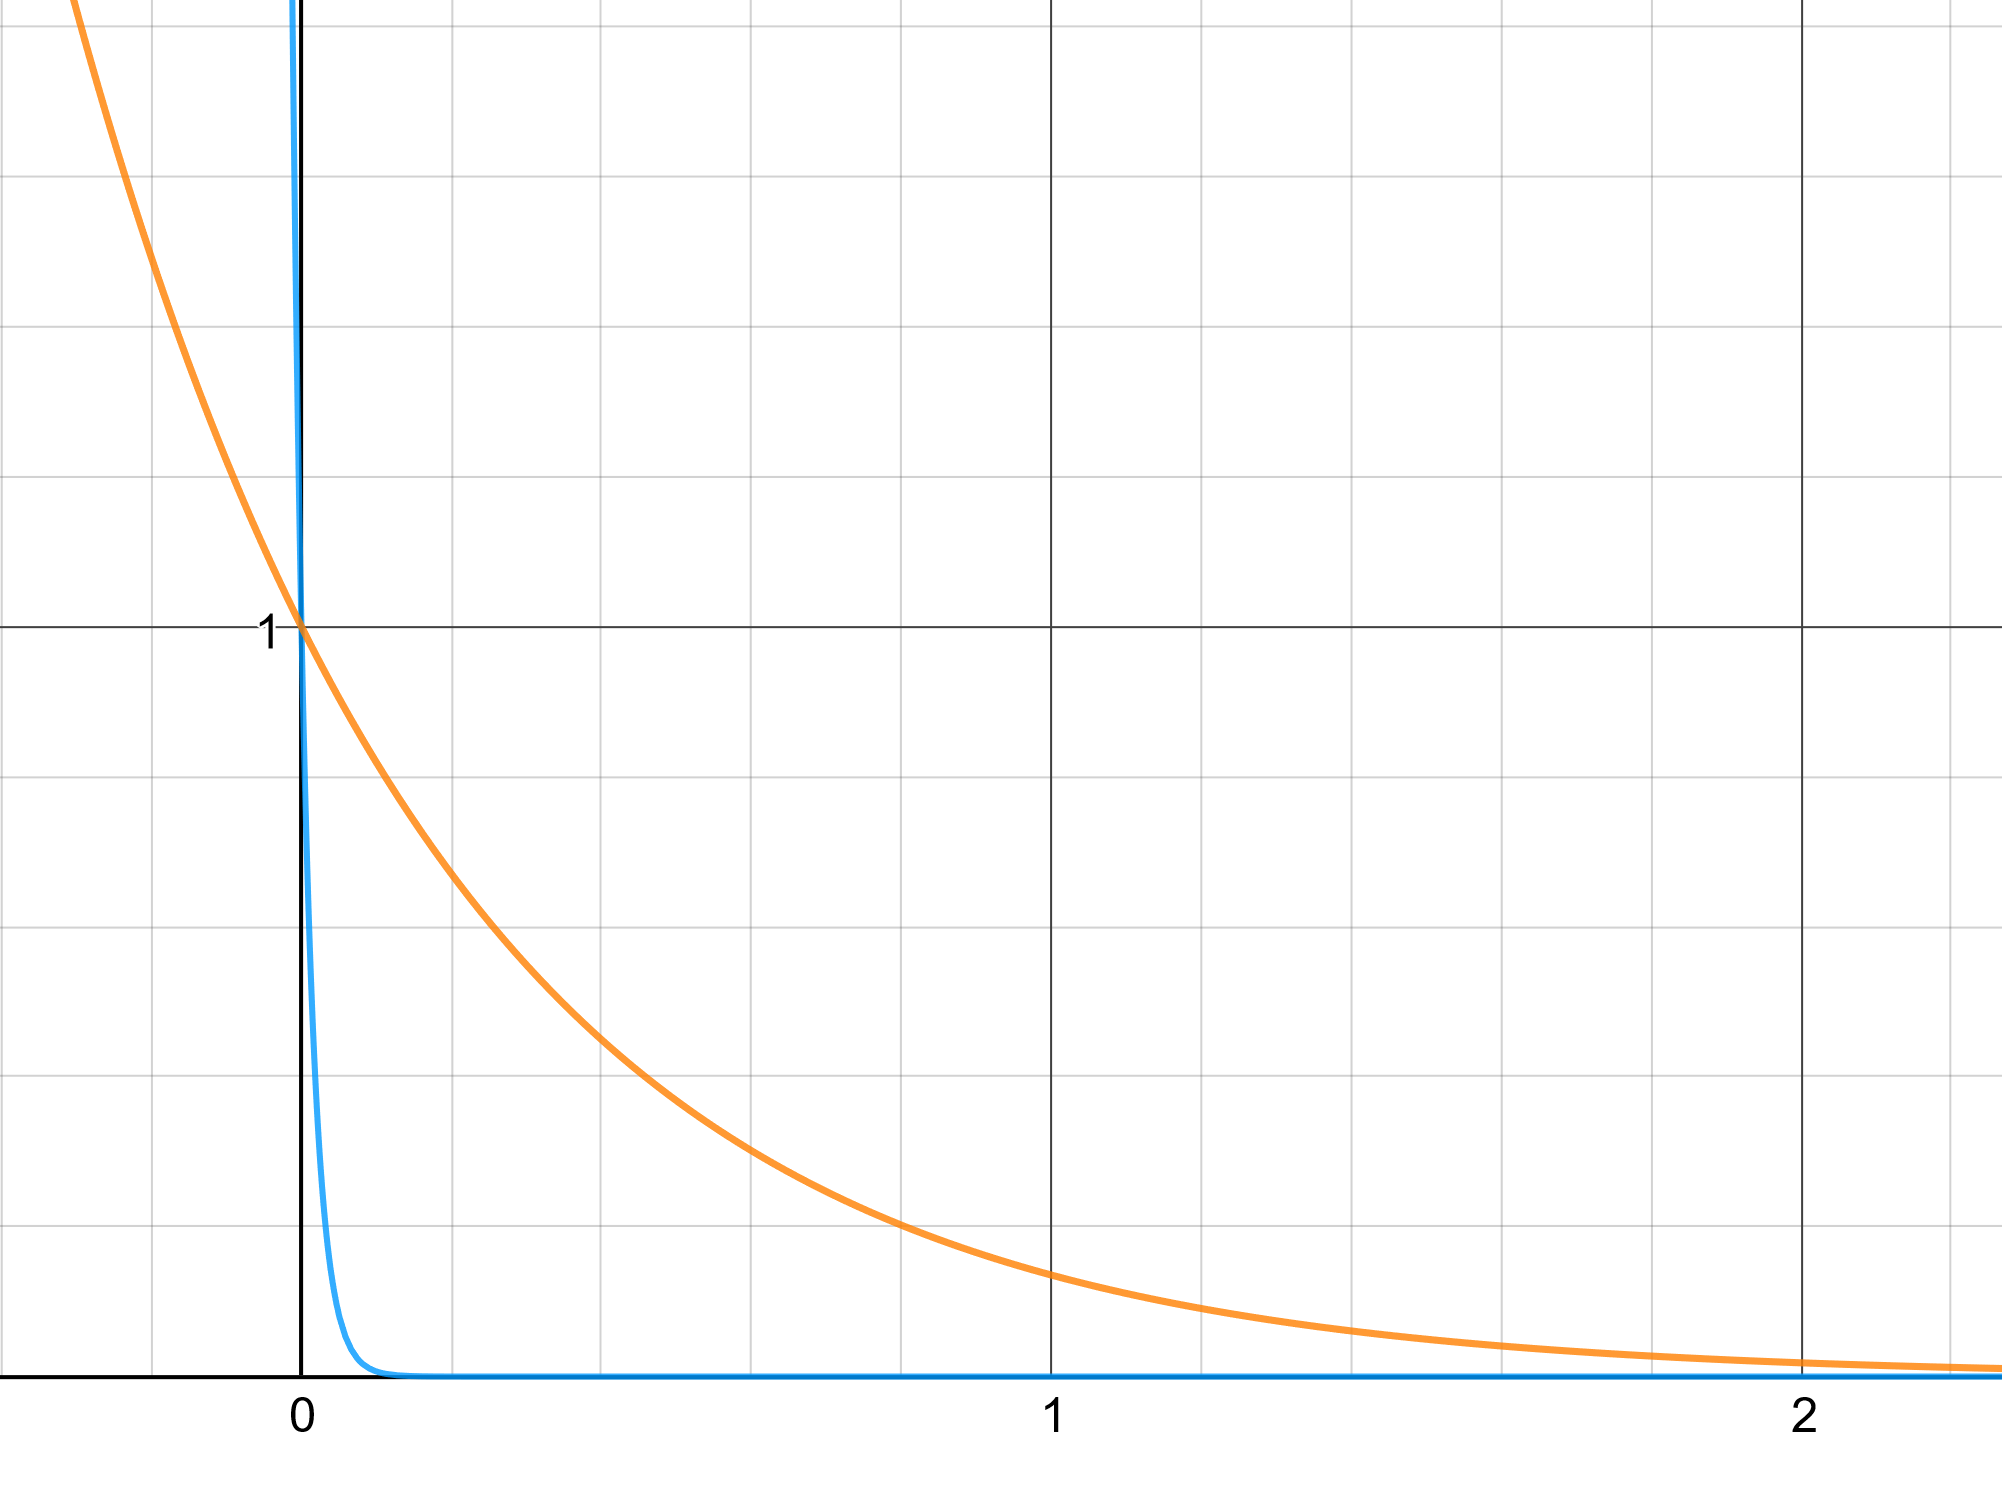
\includegraphics[width = 0.5\linewidth]{figures/e_expl_curve.png}
	\caption{Graph explaining the difference in acceptance rates (Generated at https://www.geogebra.org/graphing/g7kyzwce)}
	%TODO
	%Fix sizing
	\end{figure}
	
	To allow for sufficient number of samples the program was run until 20 000 samples were generated.
	The program was run four times with 5000 iterations each time. 
	Due to computational limitations more iterations could not be run.
	Due to burn-in, as explained in Section \ref{markovexpl}, the first 100 samples of each run was removed from analysis. 
	This resulted in 19 600 acceptable and useful samples that were analysed.
	
	
	
	\section{MAP}
The maximum a posteriori of the posteriori function was also determined to allow for further comparison of results.
All the values and constants except for the $\kappa$-values were kept the same as in the MCMC integration to allow the results to be compared on the same basis.  
	The optimisation to determine the maximum value of the posteriori function was initially done utilising the built-in Matlab optimisation algorithm \texttt{femsearchmin.m}. 
	Since the built-in optimisation intends to minimise the function the probability was multiplied with -1 such that the minimum found is truly the maximum.
	After initial analysis, the maximum was found at negative $\kappa$-values, as previously stated that is illogical and impractical.
	Further research on various adaptations of the built-in function lead to finding the \texttt{femsearchminbnd.m} adaptation by \citet{derrico:2021}. 
	This was used to limit the search area to only positive $\kappa$-values.
	Further, the algorithm was set to only iterate a thousand times and stop if the points of the simplex are within 0.009 of each other.
	The start point for the algorithm was chosen to be the $\kappa$-values from the Eurocode.
	
%	A problem that arose was that the function could get stuck at a local maximum.
%	This can be seen in Figure \ref{fig:scatdata} on the histogram for 140\textdegree C
	
	
